\documentclass{article}
\usepackage[main]{template/neurips_2026}
\usepackage[utf8]{inputenc}
\usepackage[T1]{fontenc}
\usepackage{amsmath,amssymb}
\usepackage{graphicx,booktabs,xcolor}
\usepackage{courier} % Type-1 monospaced font for reproducible settings and paths
\usepackage{hyperref,url}
\usepackage{microtype}
\newcommand{\Top}{\operatorname{Top}_3}
\newcommand{\E}{\mathbb{E}}
\newcommand{\ind}{\mathbf{1}}
\DeclareRobustCommand{\artifact}[1]{\path{#1}}
\title{When Does One Permutation SHAP Run Recover the Leading Features?\\A Fixed-Game Budget and Margin Audit of Tabular Models}
\author{Anonymous Authors}
\begin{document}
\maketitle

\begin{abstract}
A finite-budget feature attribution can satisfy additivity while failing to recover the features with the largest Shapley magnitudes. We audit this distinction for a standard paired forward/reverse permutation estimator, holding the prediction model, instance, empirical background, and grouped-feature game fixed. Across Pima diabetes, ACSIncome, and German Credit, we evaluate logistic regression, random forests, and multilayer perceptrons at three fixed training seeds, using 120 instances per dataset, 20 repetition streams, and four nested budgets. Exact enumeration supplies the target for Pima and ACS; German results measure agreement with an approximate two-pool reference, not true accuracy. Exact-game macro top-three set recovery rises from 0.7656 at one cycle to 0.9656 at 64 cycles; the additional 90 instances, held out after an exploratory first-30 analysis, yield 0.7705 and 0.9666. Descriptive paired instance-cluster intervals accompany these estimates. Nevertheless, both exact-game neural-network means remain below a user-defined 0.95 criterion at the largest budget, and small reference-gap strata remain difficult. Material-sign agreement is already high at low budget, showing that reliability depends on the question asked of an attribution. The findings characterize approximation fidelity for fixed empirical games, not causal validity, model correctness, population certification, or deployment safety.
\end{abstract}

\section{Introduction}
Feature attributions are often read as a short answer to a local question: which inputs contributed most to this prediction? SHAP connects that answer to Shapley values for a specified cooperative game \citep{lundberg2017shap}. In practice, the vector shown to a user may instead be a stochastic approximation. A single displayed explanation therefore involves two choices: what game is being explained, and how much computation is used to estimate its values. An attribution can be internally additive without its leading-feature summary being reproducible or accurate for that game.

We ask whether \emph{one} finite-budget permutation run recovers the unordered set of the three largest absolute Shapley values of a fixed prediction. Repeated runs estimate the behavior of that single-run procedure; they are not combined into its displayed output. We distinguish exact-target recovery, approximate-reference agreement, and between-run agreement. None establishes that the chosen game represents an appropriate real-world reason.

Top-three membership changes discontinuously when the third and fourth magnitudes are close: small Monte Carlo vector errors can change the selected set. Meanwhile, material positive or negative contributions may retain accurately estimated signs despite unstable ordering. An audit must distinguish these questions rather than attach one reliability label to every use of an attribution.

Our contribution is an empirical, margin-aware audit, not a new estimator or priority claim. We isolate approximation randomness across datasets and model families, quantify budget effects and metric dependence with paired instance-cluster uncertainty, and retain difficult cases: near ties, neural-network failures, background changes, and German's reference ambiguity. Figure~\ref{fig:budget} and Table~\ref{tab:nine} provide the core evidence.

Even strong observed recovery cannot establish a finite-sample population guarantee here: the instance count is limited, and ACS selection is not a justified survey-weighted design. Exact recovery validates only estimation of the fixed game, not causal effects, fairness, calibrated probabilities, predictive correctness, or safety. The illustrative 0.95 criterion is user-defined, not a medical or regulatory standard.

\section{Related work}
\paragraph{Attribution targets and approximation.}
\citet{lundberg2017shap} define additive feature explanations, give an axiomatic characterization, and connect Kernel SHAP to weighted regression. Their empirical approximation comparisons also motivate measuring variability across replicate estimates. The axioms characterize a target for a specified mapping; they do not make every finite-budget realization accurate. \citet{chen2020true} distinguish observational from interventional value functions and argue that the appropriate choice depends on the explanation goal. We explicitly select an empirical-interventional probability game. It breaks dependence between observed and background features and may query implausible hybrids; its exact Shapley vector is not observational or causal ground truth.

\paragraph{Sampling accuracy versus a selected-feature summary.}
\citet{musco2025leverage} change the sampling distribution for constrained Shapley regression using leverage scores. We read their October 2026 arXiv v3. Its guarantee concerns a regression objective under an expected-budget Bernoulli sampling algorithm; the deterministic-budget implementation used in its main experiments is not covered verbatim by that analysis. Such guarantees are not automatically guarantees of exact top-three recovery. We do not implement Leverage SHAP or benchmark optimized SHAP routines, and make no empirical superiority claim against them. Our plain constrained Kernel control diagnoses estimator sensitivity and becomes a full-enumeration control at the largest allowance on the exact datasets.

\paragraph{Stability and dataset scope.}
\citet{nogueira2018stability} develop a chance-corrected statistic for selected feature subsets. We apply it only after declaring an absolute top-three extraction rule, and distinguish approximation randomness in a fixed game from training-data resampling. We do not transfer their asymptotic inference mechanically to paired runs or repetition pairs. \citet{ding2022retiring} introduce ACS-derived tasks and emphasize geographic, temporal, and task-definition context. Our ACS experiment uses one state and year, not their national evaluation protocol. These targeted original-paper readings support our definitions and comparisons; they are not an exhaustive literature review.

\section{Methods: an audit of a fixed explanation game}
\label{sec:methods}
\subsection{Target, grouped players, and reference construction}
Let $f$ return the fitted model's positive-class probability, $x$ be a fixed test instance, and $b_1,\ldots,b_B$ be fixed training-background rows. For raw-feature players $D=\{1,\ldots,d\}$, define
\begin{equation}
 v_x(S)=\frac{1}{B}\sum_{b=1}^{B} f(x_S,b_{D\setminus S}),\qquad
 \phi_j=\sum_{S\subseteq D\setminus\{j\}}
 \frac{v_x(S\cup\{j\})-v_x(S)}{d\binom{d-1}{|S|}}.
 \label{eq:game}
\end{equation}
The link is identity, so attributions are in probability units. Each categorical variable is one player: all of its encoded columns switch together. Because imputation and encoding/scaling are fitted separately per raw feature, grouped switching after transformation implements the same game as raw-feature switching followed by transformation. Summing unconstrained dummy-column Shapley values would generally define a different game and is not used.

The primary background is the first $B=8$ rows of a fixed ordered training sample. For Pima ($d=8$) and ACS ($d=10$), we evaluate all $2^d$ coalitions and compute Eq.~\eqref{eq:game}. These are exact targets for the finite background, not exact expectations over a population. For German ($d=20$), we average two independent 512-cycle permutation-pair pools to obtain $\widetilde\phi$. The pools are independent of the evaluation streams. Pool-to-pool agreement and vector differences assess convergence, but neither provides exact truth or a formal reference-error bound. All German errors and matches are therefore \emph{approximate-reference agreement}.

\subsection{Single-run estimator and fair cost accounting}
For a uniformly random permutation $\pi$, let $A_j^\pi$ be the players preceding $j$, and write $\Delta_j(\pi)=v_x(A_j^\pi\cup\{j\})-v_x(A_j^\pi)$. One antithetic cycle pairs a permutation with its reverse:
\begin{equation}
 C_j(\pi)=\tfrac12\{\Delta_j(\pi)+\Delta_j(\operatorname{rev}\pi)\},\qquad
 \widehat\phi_{P,j}=\frac1P\sum_{p=1}^P C_j(\pi_p).
 \label{eq:estimator}
\end{equation}
This is a standard transparent custom permutation estimator. Uniform paths have the Shapley vector as their expectation, and each path telescopes to $v_x(D)-v_x(\varnothing)$. Thus efficiency is a useful correctness check but not a recovery guarantee. We use nested prefixes $P\in\{1,4,16,64\}$ within each of 20 independent repetition streams per fixed game. Dependence between budgets is intentional and retained in the analysis.

We charge logical model-row cost
\begin{equation}
 L_{\rm perm}(P)=B\{2+2P(d-1)\},\qquad L_{\rm cube}=B2^d.
 \label{eq:cost}
\end{equation}
The two common endpoints are evaluated once; repeated interior-coalition reuse is not credited. At equal logical allowance, the independent one-way control averages $2P$ unrelated permutation paths. A second control fits plain constrained Kernel regression without L1 feature selection, sampling coalition sizes with mass proportional to $1/[s(d-s)]$ and subsets uniformly within size. Endpoints fix the intercept and total attribution. When the allowance $m=2+2P(d-1)$ reaches $2^d$, this control instead uses every coalition with its Kernel weight and costs $B\min(m,2^d)$ rows. Consequently, $P=64$ is exact enumeration for both Pima and ACS, and costs \emph{less} than the nominal permutation allowance. It is not evidence of a superior randomized estimator.

Coalition values are cached within each fixed game for tractable repeated evaluation. Actual cached rows and recorded runtime include target/reference construction and shared comparison work; they cannot be assigned to individual estimators or read as deployment timing. A high-budget SHAP-package smoke check tests consistency on simple games, not speed or package-level performance. Likewise, averaging equal-sized blocks of the \emph{same} sampled cycles equals their longer-run average algebraically. We test this identity as a control, not propose repeat-and-average as a new algorithm.

\subsection{Metrics, uncertainty, and the meaning of a threshold}
Let $T(a)=\Top(|a|)$, with exact ties resolved by lower raw-feature index. Our primary outcome is $\ind\{T(\widehat\phi_P)=T(\phi)\}$; German substitutes $\widetilde\phi$. Top-three is an unordered set, not a rank-order match. Secondary outcomes are target overlap, probability-unit L1 error, L1 normalized by $\max(\|\phi\|_1,0.01)$, and agreement on the signs of target features with $|\phi_j|\geq0.01$. Sign agreement is undefined when no feature is material; valid-instance counts and the fraction of games with any material feature are retained. We also measure pairwise top-three equality and overlap within the 20 repetition streams, and Nogueira subset stability. Appendix~\ref{app:metrics} gives exact definitions.

Runs are averaged within each fixed-seed instance, then seeds within instance, then instances. The exact-game macro is an equal-weight mean over Pima/ACS $\times$ LR/RF/MLP, excluding German. The three training seeds are fixed design settings, not sampled model replicates; deterministic LR fits do not provide three independent models. Uncertainty uses 2,000 paired instance-cluster bootstrap replicates: within a dataset, all models, seeds, methods, budgets, and repetitions retain the same resampled instance indices; datasets have independent streams. Marginal intervals are the 2.5th and 97.5th percentiles. They are \emph{descriptive}, conditional on these fitted models and backgrounds, and may collapse at boundaries.

For claimed differences, we additionally report one joint max-centered-absolute-deviation bootstrap band over 63 exact-game contrasts: antithetic minus each control at every budget and $P64-P1$, for the six cells and their macro. This preserves pairing and addresses the reported contrast family, but remains descriptive rather than an exact finite-sample guarantee. The family and its correction are specified in Appendix~\ref{app:metrics}.

We compare recovery to an illustrative user-defined criterion of 0.95. A marginal lower endpoint above 0.95 is not population certification. As a conservative sample-size illustration, a one-sided Bonferroni Hoeffding lower bound across the 24 exact antithetic dataset/model/budget cells would be $\max\{0,\widehat\mu-\sqrt{\log(24/0.05)/(2n)}\}$ under justified independent-cluster or finite-pool sampling assumptions. At $n=120$, its maximum is 0.8396 even at observed perfection. ACS's unequal household selection does not establish those assumptions for survey-population inference. No universal reliability declaration is made.

Finally, we stratify exact-game outcomes by the reference gap $g=|\phi|_{(3)}-|\phi|_{(4)}$ into $[0,0.002)$, $[0.002,0.01)$, and $[0.01,\infty)$. These bins diagnose sensitivity of a discontinuous summary. They use the reference, are oracle-dependent, and cannot serve as validated deployment selectors.

\section{Experiments}
\label{sec:experiments}
\subsection{Data, frozen fits, and study chronology}
We use German Credit's raw categorical file, OpenML Pima diabetes version 1, and Folktables 0.0.12 ACSIncome for Vermont, 2018, 1-Year person records. The positives are bad credit, diabetes, and income above \$50,000, respectively. Pima zeros in glucose, blood pressure, skin thickness, insulin, and body mass are treated as missing. ACS uses the installed package's filter, including income strictly greater than \$100, rather than silently substituting a prose threshold. Preprocessing is train-only: median imputation and standardization for numeric variables, most-frequent imputation and one-hot encoding with unknown-category tolerance for categorical variables.

German and Pima use stratified nominal 60/20/20 train/validation/test splits; ACS uses household-group splits with the same nominal proportions, yielding different person counts. Exact counts, raw/encoded dimensions, and predictive performance appear in Appendix~\ref{app:data}. The external validation partitions are not used for outcome-driven tuning. The MLP separately uses internal early stopping on a fraction of its training partition. Hyperparameters are frozen: LR with $C=1$, a 40-tree depth-6 RF, and a $(32,16)$ MLP, at training seeds 11, 23, and 47. These are small controlled models, not optimized predictive benchmarks.

Each dataset has 120 fixed audit instances shared across model families and seeds. Pima and German follow a seeded permutation of test rows. ACS scans a seeded person permutation, retaining the first person from each unseen household. Although this prevents multiple audit persons from the same household, households with more eligible persons have different inclusion probabilities. All ACS intervals are therefore descriptive, not design-valid US-population or survey-weighted statements.

The original 30-instance study was exploratory. After inspecting it, we specified a uniform precision expansion of every main cell to 120 instances, before viewing expanded outcomes, keeping the ordering, models, backgrounds, metrics, thresholds, and budgets unchanged. The next 90 are held-out precision validation, not an originally preregistered independent confirmatory experiment. The first 30 replay exactly across all stored arrays in all 27 dataset/model/seed cells; model parameters, test metrics, and data manifests also match. We report the combined 120 as the main expanded analysis while retaining separate cohort summaries. The combined 120 overlaps both separate cohorts; the first 30 and next 90 are disjoint instance sets but share fitted models and backgrounds, not independent studies. The background sensitivity remains only the original first ten instances, seed 11, on the exact datasets.

\subsection{Budget improves recovery but does not eliminate failures}
\begin{table}[t]
\caption{Single-run antithetic top-three set recovery $\uparrow$ for the combined 120-instance audit. Entries are means and marginal descriptive 95\% paired instance-cluster intervals, with runs and fixed seeds averaged within instance. \textbf{German rows measure agreement with an approximate reference, not true accuracy.} Source: \artifact{analysis120/paper_antithetic_9cells.tex} and matching CSV.}
\label{tab:nine}
\centering
\resizebox{\textwidth}{!}{% Main slice n=120; positional range [0,120); marginal descriptive 95% cluster CIs, not certificates.
% Top3 subset agreement; German approximate reference ONLY.
% Top-3 subset agreement [marginal descriptive 95% instance-cluster CI]. German: approximate reference only.
\begingroup\footnotesize\setlength{\tabcolsep}{3pt}
% Requires booktabs. Machine-readable full precision: matching CSV.
\begin{tabular}{lllll}
\toprule
Game & P=1 & P=4 & P=16 & P=64 \\
\midrule
PIMA/LR & 0.853 [0.818, 0.887] & 0.926 [0.902, 0.950] & 0.965 [0.947, 0.981] & 0.981 [0.967, 0.992] \\
PIMA/RF & 0.840 [0.816, 0.863] & 0.926 [0.910, 0.940] & 0.959 [0.947, 0.970] & 0.975 [0.965, 0.983] \\
PIMA/MLP & 0.638 [0.611, 0.665] & 0.798 [0.773, 0.824] & 0.890 [0.870, 0.909] & 0.940 [0.924, 0.955] \\
ACS/LR & 0.705 [0.658, 0.752] & 0.853 [0.815, 0.887] & 0.926 [0.896, 0.950] & 0.962 [0.940, 0.980] \\
ACS/RF & 0.891 [0.872, 0.909] & 0.949 [0.935, 0.962] & 0.977 [0.969, 0.985] & 0.988 [0.981, 0.993] \\
ACS/MLP & 0.667 [0.637, 0.698] & 0.816 [0.794, 0.839] & 0.902 [0.883, 0.920] & 0.949 [0.935, 0.962] \\
GERMAN (approx.)/LR & 0.838 [0.802, 0.874] & 0.909 [0.880, 0.936] & 0.960 [0.941, 0.977] & 0.980 [0.964, 0.993] \\
GERMAN (approx.)/RF & 0.734 [0.707, 0.761] & 0.857 [0.835, 0.877] & 0.926 [0.910, 0.942] & 0.966 [0.954, 0.976] \\
GERMAN (approx.)/MLP & 0.613 [0.587, 0.637] & 0.793 [0.769, 0.816] & 0.893 [0.875, 0.911] & 0.949 [0.936, 0.962] \\
\bottomrule
\end{tabular}
\endgroup
}
\end{table}

Table~\ref{tab:nine} shows increasing recovery at every reported budget in all nine dataset/model combinations. The exact-game macro rises from 0.7656 [0.7523, 0.7790] at $P=1$ to 0.9656 [0.9597, 0.9709] at $P=64$. The paired gain is 19.998 percentage points, with a marginal interval [18.863, 21.121] and the 63-contrast simultaneous descriptive band [14.956, 25.039]. This supports a budget effect within the frozen design, not a uniform deployment guarantee. The macro at $P=16$ is 0.9366 [0.9287, 0.9440], below the illustrative criterion even at its marginal upper endpoint.

The expanded result is not solely a restatement of the inspected first 30. The held-out next 90 have exact-game macro recovery 0.7705 [0.7539, 0.7863] and 0.9666 [0.9598, 0.9735] at $P=1$ and 64. The exploratory first 30 gave 0.7511 and 0.9628. These cohort summaries characterize persistence under the fixed ordering, not two independent replications or a retrospective preregistration (Appendix~\ref{app:cohorts}).

The macro hides consequential exceptions. At $P=64$, Pima/MLP recovers the exact set with mean 0.9400 [0.9243, 0.9547], and ACS/MLP with mean 0.9490 [0.9354, 0.9618]. Both point estimates are below 0.95, while both intervals cross it; they are inconclusive relative to that threshold, not certified failures or successes. ACS/LR also has a marginal lower endpoint below 0.95. At the other extreme, ACS/RF reaches 0.9876 [0.9808, 0.9935]. This heterogeneity makes a single mean unsuitable as a budget prescription for every fitted prediction.

\begin{figure}[t]
\centering
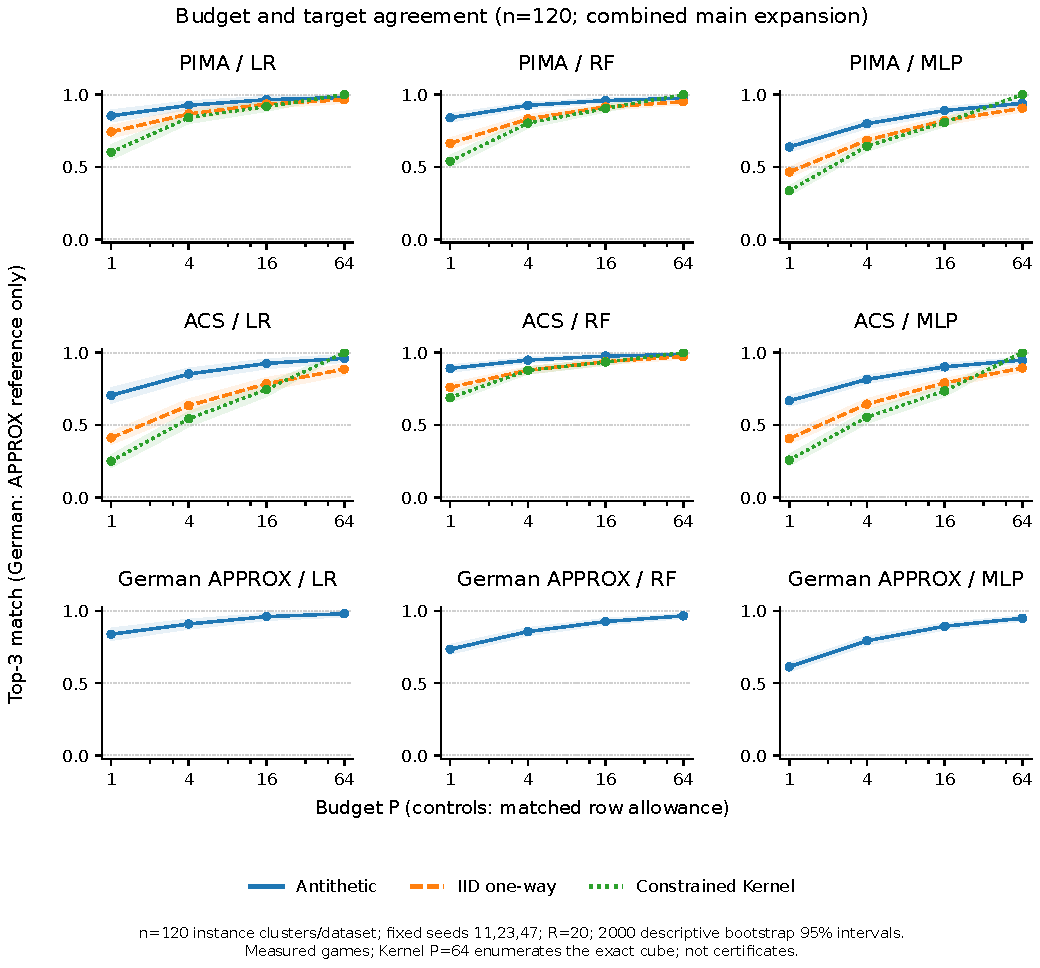
\includegraphics[width=\textwidth]{analysis120/budget_accuracy.pdf}
\caption{Budget and leading-feature recovery, with descriptive 95\% instance-cluster bands. Pima and ACS use exact targets; German uses approximate-reference agreement. Controls share a row \emph{allowance}: Kernel at $P=64$ enumerates both exact cubes using fewer rows than permutation. These are custom-estimator recovery curves, not package timings. Artifact: \artifact{analysis120/budget_accuracy.pdf}.}
\label{fig:budget}
\end{figure}

\subsection{Controls delimit the estimator comparison}
\begin{table}[t]
\caption{Exact-game macro top-three recovery $\uparrow$ over six Pima/ACS model cells. Marginal descriptive 95\% paired cluster intervals. Kernel's $P=64$ entry is a \emph{full-cube exact control}, not a sampled-estimator result; its collapsed interval is not a population certificate. Source: \artifact{analysis120/paper_exact_macro_controls.tex}.}
\label{tab:controls}
\centering
\resizebox{\textwidth}{!}{% Main slice n=120; positional range [0,120); marginal descriptive 95% cluster CIs, not certificates.
% Six exact dataset/model cells; Kernel P64 fully enumerates both cubes (not sampled).
\begingroup\footnotesize\setlength{\tabcolsep}{3pt}
% Requires booktabs. Machine-readable full precision: matching CSV.
\begin{tabular}{lllll}
\toprule
Method & P=1 & P=4 & P=16 & P=64 \\
\midrule
antithetic & 0.766 [0.752, 0.779] & 0.878 [0.867, 0.888] & 0.937 [0.929, 0.944] & 0.966 [0.960, 0.971] \\
iid\_oneway & 0.575 [0.560, 0.590] & 0.757 [0.743, 0.770] & 0.864 [0.854, 0.875] & 0.929 [0.921, 0.937] \\
kernel & 0.445 [0.429, 0.461] & 0.710 [0.695, 0.725] & 0.842 [0.829, 0.853] & 1.000 [1.000, 1.000] \\
\bottomrule
\end{tabular}
\endgroup
}
\end{table}

At $P=1$, antithetic pairing has higher observed macro recovery than the equal-row independent one-way control: 0.7656 versus 0.5747 (Table~\ref{tab:controls}). The difference is 19.100 percentage points, marginal interval [18.032, 20.144], simultaneous band [14.058, 24.141]. This identifies the benefit of the pairing in these games, not a new algorithm. At $P=64$, the corresponding 3.641-point difference has a simultaneous band spanning zero, [--1.400, 8.683]; marginal intervals alone would overstate the corrected comparison.

Plain sampled Kernel regression has lower recovery at the smaller allowances in this implementation, but its largest-budget exact control reaches 1.0000 on both datasets. It is also cheaper than the nominal permutation run at that allowance: 2,048 versus 7,184 logical model rows for Pima, and 8,192 versus 9,232 for ACS. Exact enumeration is thus an important practical option in these small games, not merely an expensive abstract target. These controls do not justify comparing our custom code favorably to optimized Kernel SHAP or Leverage SHAP. The model-class and game restrictions are as important as the apparent sampling curves.

\subsection{Near ties and metric dependence explain residual fragility}
\begin{figure}[t]
\centering
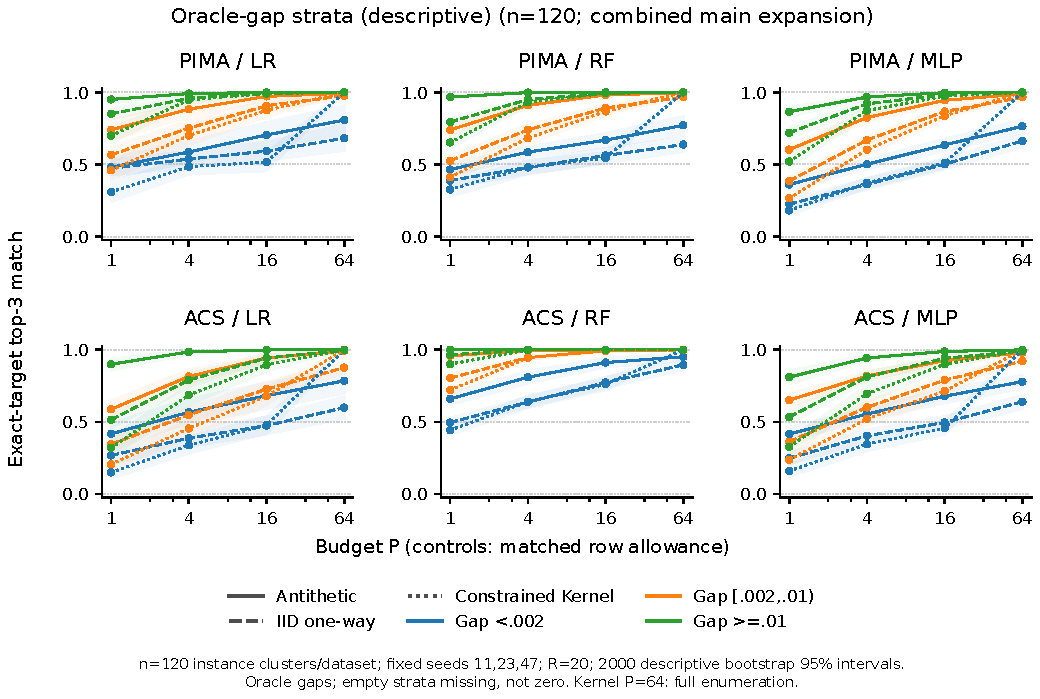
\includegraphics[width=\textwidth]{analysis120/gap_budget.pdf}
\caption{Exact-game recovery conditional on the \emph{reference} rank-three/rank-four magnitude gap. Small-gap strata remain difficult at high aggregate recovery. Bands are descriptive paired cluster intervals for stratum ratios; Appendix~\ref{app:gaps} gives counts. These oracle-dependent bins are not deployable confidence rules. Artifact: \artifact{analysis120/gap_budget.pdf}.}
\label{fig:gap}
\end{figure}

The residual errors are concentrated in reference near ties (Figure~\ref{fig:gap}). At $P=64$, Pima/MLP recovery is 0.7647 [0.7211, 0.8089] in the $g<0.002$ stratum, but 1.0000 [1.0000, 1.0000] for $g\geq0.01$. ACS/MLP gives 0.7790 [0.7330, 0.8228] and 0.9993 [0.9981, 1.0000], respectively. This is a conditional diagnosis, not evidence that every failure has the same cause: the strata contain different fixed games and are not randomized interventions on the gap. Their target-dependent membership also precludes using these numbers directly to select a budget without a reference.

Other summaries tell a much more favorable story at low budget. Exact-game macro material-sign agreement is already 0.9983 [0.9980, 0.9986] at $P=1$, despite top-three recovery of only 0.7656. For Pima/MLP alone, those means are 0.9933 and 0.6379. Sign recovery concerns only target features above the declared magnitude threshold; it does not require discovering which three features are largest or representing small contributions faithfully. At $P=64$, exact-game macro material-sign agreement is 1.0000, but exact-set recovery is still imperfect. Reliability is therefore metric-dependent, not an intrinsic binary property of a plotted attribution.

Vector and repeatability summaries reinforce this distinction. Exact-game macro L1 error decreases from 0.039883 to 0.004718 probability units, while pairwise top-three equality increases from 0.6970 to 0.9528. Nogueira stability increases from 0.8395 to 0.9762. The latter exceeds exact-set recovery numerically because it is a different, chance-corrected subset functional, not a probability of correctness. Figure~\ref{fig:repeatability} in the appendix juxtaposes repeatability and target recovery without treating one as a calibrated predictor of the other. Repetition pairs never increase the inferential sample size.

\subsection{Reference convergence and background sensitivity}
German's independent reference pools have top-three agreement 0.9917 for LR, 0.9806 for RF, and 0.9778 for MLP, with mean pool L1 differences 0.003063, 0.002465, and 0.005204 probability units (Appendix~\ref{app:german}). These diagnostics indicate close but imperfect convergence. At $P=64$, German/MLP has approximate-reference agreement 0.9493 [0.9358, 0.9617]. We retain it and every pool disagreement; we neither relabel the pooled target as exact nor discard ambiguous games to manufacture recovery.

Background sensitivity answers a different question from increasing the approximation budget. Replacing the eight-row background with the nested sixteen-row background changes the target top-three set in 5/10, 5/10, and 4/10 Pima instances for LR/RF/MLP, and 9/10, 5/10, and 7/10 ACS instances. At $P=64$, own-target Pima/MLP recovery changes from 1.000 to 0.985, whereas ACS/MLP changes from 0.930 to 0.960. These small first-ten, seed-11 comparisons have paired descriptive intervals in Appendix~\ref{app:sensitivity}. More background rows do not uniformly improve recovery, and they do not merely make the same estimand more accurate: they define another empirical game.

\section{Discussion and limitations}
\label{sec:discussion}
The supported answer to the motivating question is conditional. A single paired permutation run can recover the leading features frequently at sufficiently large budgets in some fixed empirical games. It is not uniformly reliable across fitted models or close ranking boundaries, and low-budget sign accuracy cannot validate an exact-set interpretation. An audit should state the output scale, background, player grouping, target, and downstream summary before deciding which form of agreement matters. Where a small coalition cube is affordable, the exact-control results argue for considering enumeration rather than assuming random approximation is necessary.

\paragraph{Statistical limits.}
The bootstrap quantifies instance-cluster variation conditional on fixed models and backgrounds. It is not an exact confidence procedure, can be degenerate at perfect agreement, and does not make three fixed seeds into an estimate of training-distribution uncertainty. The simultaneous bands address only the reported 63-contrast family. The precision expansion followed inspected exploratory results; retained cohorts and frozen prefixes make that history auditable, but do not erase it. For ACS, household-disjoint splits prevent household overlap across partitions, while person-permutation deduplication still induces unequal household audit inclusion. Neither the bootstrap nor the Hoeffding illustration repairs that design. We make no US-population claim.

\paragraph{Scientific and computational limits.}
Only three modest model families, one background realization per dataset, and one state/year of ACS are tested. The MLP fits are not uniformly good predictors: Pima seed 23 has test AUC 0.4826, and German seed 23 has AUC 0.5711; both are retained. Approximation fidelity does not rescue a weak model. No subgroup fairness, temporal transfer, probability calibration, human usefulness, or causal assessment is established. Interventional hybrids may be off-manifold. German's pooled reference leaves unquantified residual target error, and a summed dummy-column TreeSHAP shortcut was rejected because it would change the grouped-player game.

Cached computation makes the controlled audit feasible but is not a latency benchmark. Successful original and expanded campaigns consumed a measured 0.3319 CPU hours in total, including prefix replay; failed-run overhead and historical CPU identity were not recorded. Logical costs are more transferable than these shared timings. We did not evaluate optimized SHAP estimators or Leverage SHAP. The pandas StringDtype failure was corrected and regression-tested before completing German cells; it was an implementation failure, not an unfavorable result removed from analysis (Appendix~\ref{app:checks}).

\paragraph{Implications and next steps.}
Calling an explanation ``reliable'' without its metric risks unwarranted confidence in consequential settings. Our findings do not authorize clinical or credit decisions, individual recourse, or a safety interpretation of 0.95 agreement. Priorities are a prespecified equal-probability or design-weighted ACS audit, more independent instances if certification is sought, larger independent German reference pools, and validation of a reference-free budget diagnostic. Each would address a present boundary rather than convert the current descriptive results into a deployment guarantee.

\section{Conclusion}
A fixed-game audit separates approximation fidelity from the broader validity of an explanation. In the combined 120-instance study, exact-game macro top-three recovery increases from 0.7656 to 0.9656 across the tested budgets, and the held-out next 90 retain this pattern. Yet MLP means remain below the illustrative 0.95 criterion, small reference gaps remain difficult, and strong material-sign agreement does not imply exact leading-feature recovery. German reference agreement and background changes require separate interpretations. The result is evidence for explicit, metric- and game-specific auditing of a single stochastic explanation, not a new estimator, universal certification, or real-world causal or safety validation.

\clearpage
\bibliographystyle{plainnat}
\bibliography{references}
\clearpage
\appendix

\section{Data, predictive performance, and preprocessing}
\label{app:data}
Table~\ref{tab:data} reports the actual frozen splits, rather than inferring person counts from nominal proportions. Pima has 652 missing entries after the declared zero-to-missing conversion and no duplicated raw feature rows. ACS has no missing feature entries and 79 duplicated feature rows; these are retained, not assumed to be duplicate people. German has no missing entries or duplicated raw feature rows. These QC counts are in \artifact{analysis120/data_splits.csv}. Array finiteness, unique audit row IDs, train-only backgrounds, test-only audit IDs, disjoint splits, and household-cluster uniqueness are checked by the analysis validation. Checksummed acquisition manifests reside in \artifact{data/manifest.json}; split indices, ordered backgrounds, feature lists, and audit IDs are in \artifact{results120/data_*.json}.

\begin{table}[h]
\caption{Actual dataset sizes and frozen partitions. Positive fractions describe the entire filtered dataset, not split-specific proportions. ACS partitions are household-disjoint, not stratified person splits. Source: \artifact{analysis120/paper_data_splits.tex}.}
\label{tab:data}\centering
% Main slice n=120; positional range [0,120); marginal descriptive 95% cluster CIs, not certificates.
% Frozen splits; ACS household-disjoint but audit inclusion is unequal-probability, not survey-weighted.
\begingroup\footnotesize\setlength{\tabcolsep}{3pt}
% Requires booktabs. Machine-readable full precision: matching CSV.
\begin{tabular}{lllllll}
\toprule
dataset & total\_n & train\_n & validation\_n & test\_n & Raw/encoded d & Positive \% \\
\midrule
pima & 768 & 460 & 154 & 154 & 8/8 & 34.90 \\
acs & 3767 & 2250 & 773 & 744 & 10/478 & 34.32 \\
german & 1000 & 600 & 200 & 200 & 20/61 & 30.00 \\
\bottomrule
\end{tabular}
\endgroup

\end{table}

The Pima raw fields are \texttt{preg, plas, pres, skin, insu, mass, pedi, age}. Its positive label is \texttt{tested\_positive}; missingness is introduced for zeros only in \texttt{plas, pres, skin, insu, mass}. German has 20 raw players and 13 categorical variables, with bad credit (class 2) positive. ACSIncome uses \texttt{AGEP, COW, SCHL, MAR, OCCP, POBP, RELP, WKHP, SEX, RAC1P}; the categorical variables are \texttt{COW, MAR, OCCP, POBP, RELP, SEX, RAC1P}. The code retains the ACS household identifier \texttt{SERIALNO} for splitting, not as a predictor. The package filter used in the experiment is age $>16$, income $>100$, usual hours $>0$, and person weight $\geq1$. Models and explanation averages are not survey-weighted.

\paragraph{Frozen training settings.}
The numerical imputer uses the training median, followed by per-feature StandardScaler. Categorical variables use training most-frequent imputation and dense OneHotEncoder with \texttt{handle\_unknown='ignore'}. Models see the resulting numeric matrix. LR uses \texttt{C=1}, \texttt{max\_iter=1000}, and the declared \texttt{random\_state}. RF uses \texttt{n\_estimators=40}, \texttt{max\_depth=6}, \texttt{min\_samples\_leaf=4}, and \texttt{n\_jobs=1}. MLP uses hidden layers $(32,16)$, \texttt{alpha=.01}, \texttt{max\_iter=350}, \texttt{early\_stopping=True}, \texttt{validation\_fraction=.15}, and \texttt{n\_iter\_no\_change=20}. Other settings are scikit-learn defaults for the recorded environment, with complete resolved parameters in each JSON sidecar. The MLP's internal validation subset is drawn only from training rows; the separate external validation set is unused for tuning. Neither probability calibration nor architecture search is performed.

\begin{table}[p]
\caption{Predictive metrics on the entire fixed test partition, not only the audit instances. AUC $\uparrow$, log loss $\downarrow$, and accuracy $\uparrow$ at probability threshold 0.5. These are observed fixed-test metrics; prediction-level intervals cannot be recovered from the aggregate performance table. Empty lists denote no captured fit warning. All fits, including weak MLP fits, are retained. Source: \artifact{analysis120/paper_model_performance.tex}.}
\label{tab:performance}\centering
% Main slice n=120; positional range [0,120); marginal descriptive 95% cluster CIs, not certificates.
% Frozen model performance on entire fixed test split; no prediction-level CI available.
\begingroup\footnotesize\setlength{\tabcolsep}{3pt}
% Requires booktabs. Machine-readable full precision: matching CSV.
\begin{tabular}{lllllll}
\toprule
dataset & model & seed & auc & log\_loss & accuracy & fit\_warnings \\
\midrule
pima & lr & 11 & 0.7606 & 0.5714 & 0.6883 & [] \\
pima & lr & 23 & 0.7606 & 0.5714 & 0.6883 & [] \\
pima & lr & 47 & 0.7606 & 0.5714 & 0.6883 & [] \\
pima & rf & 11 & 0.7509 & 0.5574 & 0.6818 & [] \\
pima & rf & 23 & 0.7344 & 0.5666 & 0.6818 & [] \\
pima & rf & 47 & 0.7478 & 0.5618 & 0.6883 & [] \\
pima & mlp & 11 & 0.7381 & 0.5622 & 0.6948 & [] \\
pima & mlp & 23 & 0.4826 & 0.6483 & 0.6753 & [] \\
pima & mlp & 47 & 0.7626 & 0.5668 & 0.6948 & [] \\
acs & lr & 11 & 0.8364 & 0.4745 & 0.7823 & [] \\
acs & lr & 23 & 0.8364 & 0.4745 & 0.7823 & [] \\
acs & lr & 47 & 0.8364 & 0.4745 & 0.7823 & [] \\
acs & rf & 11 & 0.7863 & 0.5619 & 0.6855 & [] \\
acs & rf & 23 & 0.8040 & 0.5580 & 0.6815 & [] \\
acs & rf & 47 & 0.8212 & 0.5517 & 0.6801 & [] \\
acs & mlp & 11 & 0.8387 & 0.4861 & 0.7809 & [] \\
acs & mlp & 23 & 0.8263 & 0.4801 & 0.7782 & [] \\
acs & mlp & 47 & 0.8270 & 0.4818 & 0.7755 & [] \\
german & lr & 11 & 0.8060 & 0.4819 & 0.7700 & [] \\
german & lr & 23 & 0.8060 & 0.4819 & 0.7700 & [] \\
german & lr & 47 & 0.8060 & 0.4819 & 0.7700 & [] \\
german & rf & 11 & 0.7840 & 0.5145 & 0.7550 & [] \\
german & rf & 23 & 0.7963 & 0.5074 & 0.7300 & [] \\
german & rf & 47 & 0.8044 & 0.5086 & 0.7550 & [] \\
german & mlp & 11 & 0.7604 & 0.5217 & 0.7700 & [] \\
german & mlp & 23 & 0.5711 & 0.6134 & 0.7100 & [] \\
german & mlp & 47 & 0.7913 & 0.4955 & 0.8000 & [] \\
\bottomrule
\end{tabular}
\endgroup

\end{table}
Table~\ref{tab:performance} records every seed fit. The identical LR test metrics reflect deterministic fits under these settings, not independent confirmations. Per-seed attribution means and descriptive intervals, without pooling seeds as independent observations, are available in \artifact{analysis120/per_seed.csv}.

\section{Metric definitions and paired inference}
\label{app:metrics}
For a fixed seed-instance game let $\widehat\phi_r$ be repetition $r$, $Z_{rj}=\ind\{j\in T(\widehat\phi_r)\}$, and $T^*=T(\phi)$ (or $T(\widetilde\phi)$ for German). The implemented summaries are:
\begin{align}
 M&=\frac1R\sum_r\ind\{T(\widehat\phi_r)=T^*\}, &
 O&=\frac1R\sum_r\frac{|T(\widehat\phi_r)\cap T^*|}{3},\\
 Q&=\binom R2^{-1}\sum_{r<s}\ind\{T(\widehat\phi_r)=T(\widehat\phi_s)\}, &
 O_{\rm pair}&=\binom R2^{-1}\sum_{r<s}\frac{|T(\widehat\phi_r)\cap T(\widehat\phi_s)|}{3},\\
 A&=\frac1R\sum_r\|\widehat\phi_r-\phi\|_1, &
 A_{\rm norm}&=\frac{A}{\max(\|\phi\|_1,0.01)}.
\end{align}
The within-game probability-unit L1 denominator is fixed across repetitions. Its normalization is applied before averaging games. Material sign agreement averages $\ind\{\operatorname{sign}(\widehat\phi_{rj})=\operatorname{sign}(\phi_j)\}$ over runs and $j$ with $|\phi_j|\geq0.01$. It is undefined for games without material features. The implementation averages available seeds within instance and then valid instances equally, retaining the fraction of games with at least one material feature and valid counts. Low-signal status is $\|\phi\|_1<0.01$, not an exclusion from recovery.

With $p_j=R^{-1}\sum_rZ_{rj}$ and $q=3/d$, the Nogueira subset statistic is
\begin{equation}
 \widehat\Phi=1-\frac{d^{-1}\sum_j[R/(R-1)]p_j(1-p_j)}{q(1-q)}.
\end{equation}
It is computed separately in each fixed game and never clipped; finite-sample values may be negative. Our selected-set size is always three, so the empty/full-set degeneracies do not arise. We report this functional descriptively and use instance-cluster bootstrapping, not the original independent-selection asymptotic test applied to 190 dependent repetition pairs. Efficiency residual is the absolute difference between estimated and target total attribution; the raw experiment also stores each instance's maximum antithetic residual.

\paragraph{Aggregation and resampling.}
For an ordinary metric $h$, the cell mean is $n^{-1}\sum_i3^{-1}\sum_s h_{is}$, where the repetition reduction is already inside $h_{is}$. The exact macro averages these means over six dataset/model cells. The same bootstrap row indices resample all $h_{is}$ within each dataset, preserving seed, model, method, and budget dependencies. Gap summaries are ratios over the seed-instance games in a bin; every bootstrap replicate recomputes the ratio after resampling instances. Counts of games and contributing clusters differ, and a cluster can contribute games to more than one stratum. Undefined ratios are omitted and counted, not replaced by zero.

For contrasts $\widehat\delta_\ell$, $\ell=1,\ldots,63$, let $\widehat\delta^{*(b)}_\ell$ be their paired bootstrap values. The correction uses
\begin{equation}
 c_{.95}=\operatorname{quantile}_{.95}\left\{
 \max_{\ell}|\widehat\delta^{*(b)}_\ell-\widehat\delta_\ell|\right\}_{b=1}^{2000},\qquad
 [\widehat\delta_\ell-c_{.95},\widehat\delta_\ell+c_{.95}].
\end{equation}
There are nine contrasts for each of six exact dataset/model cells plus the macro: two control differences at four budgets and one antithetic $P64-P1$ difference. Reported band endpoints are restricted to the feasible difference range $[-1,1]$. No studentization or finite-sample coverage claim is made. All point estimates, marginal intervals, corrected bands, and joint draws are in \artifact{analysis120/paired_comparisons.csv} and \artifact{analysis120/contrast_bootstrap.npz}. Cell, seed, and gap marginal intervals are not simultaneous certification bounds.

\begin{table}[t]
\caption{Exact-game antithetic macro secondary metrics, generated from \artifact{analysis120/exact_macro.csv}. Entries are means [descriptive 95\% paired cluster intervals]. Sign recovery and stability are not substitutes for exact top-three recovery.}
\label{tab:metrics}\centering
\begingroup\footnotesize
\begin{tabular}{lllll}
\toprule
Metric & $P=1$ & $P=4$ & $P=16$ & $P=64$ \\
\midrule
L1 $\downarrow$ & \shortstack{0.0399\\{[0.0376, 0.0423]}} & \shortstack{0.0192\\{[0.0181, 0.0203]}} & \shortstack{0.0095\\{[0.0089, 0.0100]}} & \shortstack{0.0047\\{[0.0045, 0.0050]}} \\
Normalized L1 $\downarrow$ & \shortstack{0.1182\\{[0.1140, 0.1226]}} & \shortstack{0.0571\\{[0.0551, 0.0592]}} & \shortstack{0.0283\\{[0.0273, 0.0293]}} & \shortstack{0.0141\\{[0.0136, 0.0146]}} \\
Material sign $\uparrow$ & \shortstack{0.9983\\{[0.9980, 0.9986]}} & \shortstack{0.9999\\{[0.9998, 0.9999]}} & \shortstack{1.0000\\{[1.0000, 1.0000]}} & \shortstack{1.0000\\{[1.0000, 1.0000]}} \\
Pair match $\uparrow$ & \shortstack{0.6970\\{[0.6812, 0.7124]}} & \shortstack{0.8336\\{[0.8211, 0.8456]}} & \shortstack{0.9123\\{[0.9027, 0.9216]}} & \shortstack{0.9528\\{[0.9453, 0.9597]}} \\
Stability $\uparrow$ & \shortstack{0.8395\\{[0.8308, 0.8477]}} & \shortstack{0.9151\\{[0.9087, 0.9213]}} & \shortstack{0.9557\\{[0.9508, 0.9603]}} & \shortstack{0.9762\\{[0.9725, 0.9797]}} \\
\bottomrule
\end{tabular}
\endgroup

\end{table}
Table~\ref{tab:metrics} includes vector, sign, and repeatability summaries. For each metric, \artifact{analysis120/cell_summary.csv} supplies cellwise means, intervals, valid-instance counts, low-signal fractions, and availability of at least one material feature per game (the legacy CSV field \texttt{material\_feature\_coverage}). In particular, the near-perfect sign result does not include games with no material features in its denominator. The exact-game fraction of seed-instance games with at least one material feature is 0.999537 (2,159/2,160 games), and its low-signal fraction is zero; this is not feature-level coverage.

\begin{figure}[p]
\centering
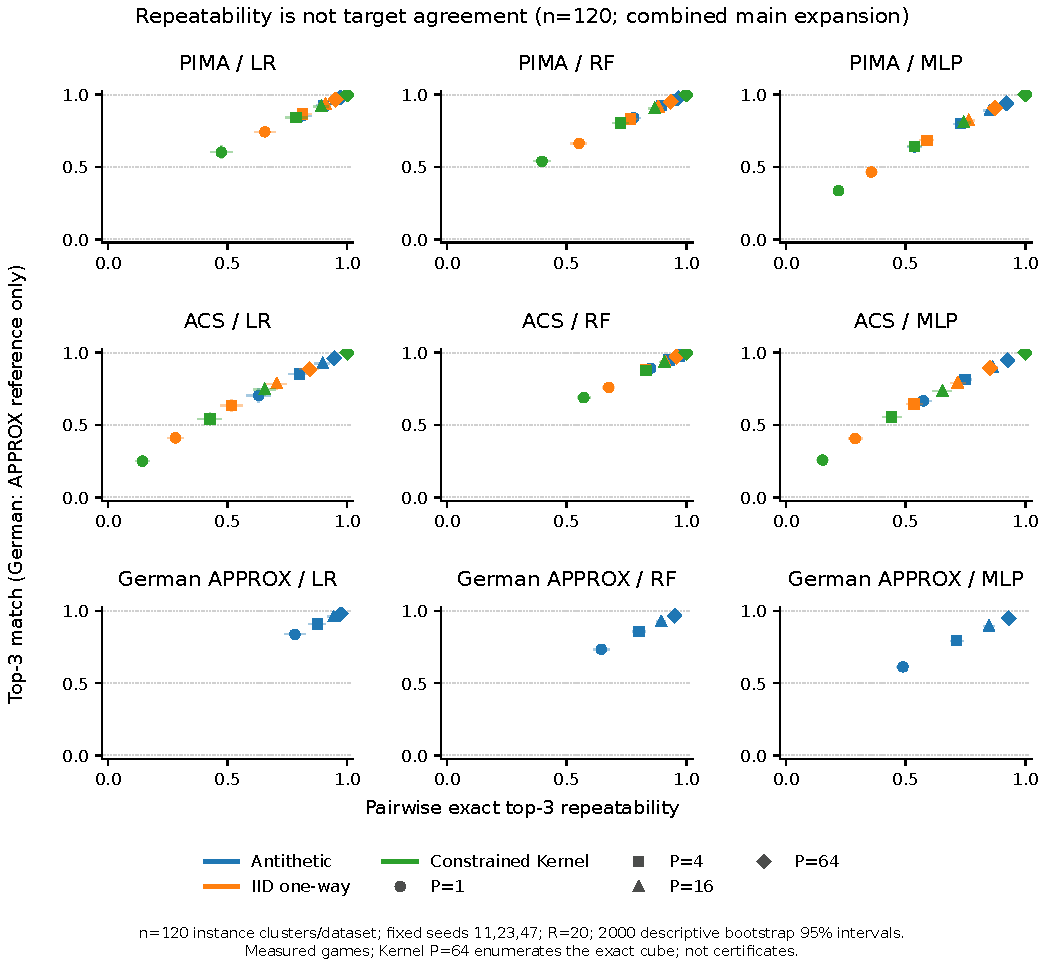
\includegraphics[width=\textwidth]{analysis120/repeatability_accuracy.pdf}
\caption{Repeatability and target agreement are different measured functionals. Horizontal coordinates are pairwise exact top-three equality within repetition streams; vertical coordinates are top-three target agreement. Intervals retain paired instance clusters, not independent pairs. German panels use an approximate reference. No fitted calibration relation or deployment rule is inferred. Artifact: \artifact{analysis120/repeatability_accuracy.pdf}; replay: \artifact{analysis120/repeatability_accuracy/plot.py}.}
\label{fig:repeatability}
\end{figure}

\paragraph{Illustrative threshold and sample size.}
The Hoeffding calculation uses bounded per-instance means, not independent repetition outcomes. The penalty at $n=120$ is 0.160387; the largest lower bound at perfection is 0.839613. At least 1,235 independent instances would be required for this particular 24-cell bound to reach 0.95 at observed perfection, under its sampling assumptions. This is not a power calculation for all alternative procedures, a promise of success at that sample size, or a justified ACS certificate. The bootstrap's potentially collapsed [1,1] interval and this conservative lower bound answer different questions.

\section{Expanded and exploratory cohorts}
\label{app:cohorts}
\begin{table}[h]
\caption{Exact-game antithetic macro by cohort and budget. The next 90 are held-out precision validation following inspection of the first 30; combined 120 overlaps both cohorts. Marginal descriptive intervals are bootstrapped at each cohort's actual instance count. Source: \artifact{analysis120/expansion_cohort_headlines.csv}.}
\label{tab:cohorts}\centering
\begingroup\footnotesize
\begin{tabular}{llll}
\toprule
Cohort & $n$ & $P$ & Exact-game macro match [95\% CI] \\
\midrule
Exploratory first 30 & 30 & 1 & 0.7511 [0.7231, 0.7787] \\
Exploratory first 30 & 30 & 4 & 0.8693 [0.8489, 0.8880] \\
Exploratory first 30 & 30 & 16 & 0.9295 [0.9148, 0.9433] \\
Exploratory first 30 & 30 & 64 & 0.9628 [0.9526, 0.9724] \\
Held-out next 90 & 90 & 1 & 0.7705 [0.7539, 0.7863] \\
Held-out next 90 & 90 & 4 & 0.8810 [0.8688, 0.8933] \\
Held-out next 90 & 90 & 16 & 0.9389 [0.9301, 0.9481] \\
Held-out next 90 & 90 & 64 & 0.9666 [0.9598, 0.9735] \\
Combined 120 & 120 & 1 & 0.7656 [0.7523, 0.7790] \\
Combined 120 & 120 & 4 & 0.8781 [0.8675, 0.8882] \\
Combined 120 & 120 & 16 & 0.9366 [0.9287, 0.9440] \\
Combined 120 & 120 & 64 & 0.9656 [0.9597, 0.9709] \\
\bottomrule
\end{tabular}
\endgroup

\end{table}
Table~\ref{tab:cohorts} preserves the chronology in \artifact{precision_expansion.md}. The original first-30 results remain under \artifact{analysis/} and \artifact{analysis30/}; expanded main and next-90 summaries are \artifact{analysis120/summary.json} and \artifact{analysis90/summary.json}. The prefix audit uses exact array equality, not a numerical tolerance chosen after inspection. All NPZ arrays, frozen model parameters, predictive metrics, split/background manifests, and deterministic prefix counters pass; timing equality is not expected. Output shape and metadata validation occur on all 120 source instances before any positional slicing.

\section{Reference-gap strata}
\label{app:gaps}
\begin{table}[p]
\caption{Antithetic exact-game top-three recovery $\uparrow$ by oracle reference-gap stratum. Games count seed-instance combinations; clusters count contributing instances. Each dataset/model has 120 audit instances and three fixed seeds, not 360 independent observations. Marginal intervals are descriptive bootstrap ratios. Source: \artifact{analysis120/paper_gaps_per_budget.tex}.}
\label{tab:gaps}\centering
\resizebox{\textwidth}{!}{% Main slice n=120; positional range [0,120); marginal descriptive 95% cluster CIs, not certificates.
% Antithetic oracle rank3-rank4 reference-gap strata; games/clusters counts; undefined strata marked --.
\begingroup\footnotesize\setlength{\tabcolsep}{3pt}
% Requires booktabs. Machine-readable full precision: matching CSV.
\begin{tabular}{lllllll}
\toprule
Game & Gap & Games/clusters & P=1 & P=4 & P=16 & P=64 \\
\midrule
PIMA/LR & <.002 & 33/11 & 0.480 [0.409, 0.546] & 0.586 [0.517, 0.658] & 0.705 [0.622, 0.790] & 0.808 [0.705, 0.906] \\
PIMA/LR & .002-.01 & 93/31 & 0.740 [0.670, 0.806] & 0.883 [0.833, 0.927] & 0.972 [0.944, 0.992] & 0.994 [0.984, 1.000] \\
PIMA/LR & >=.01 & 234/78 & 0.951 [0.928, 0.972] & 0.991 [0.983, 0.998] & 0.999 [0.997, 1.000] & 1.000 [1.000, 1.000] \\
PIMA/RF & <.002 & 38/36 & 0.464 [0.427, 0.503] & 0.586 [0.552, 0.621] & 0.668 [0.623, 0.714] & 0.771 [0.705, 0.832] \\
PIMA/RF & .002-.01 & 118/76 & 0.739 [0.709, 0.769] & 0.910 [0.886, 0.931] & 0.982 [0.973, 0.990] & 0.997 [0.995, 0.999] \\
PIMA/RF & >=.01 & 204/109 & 0.967 [0.957, 0.977] & 0.998 [0.997, 0.999] & 1.000 [1.000, 1.000] & 1.000 [1.000, 1.000] \\
PIMA/MLP & <.002 & 85/66 & 0.361 [0.329, 0.393] & 0.501 [0.469, 0.533] & 0.635 [0.596, 0.675] & 0.765 [0.721, 0.809] \\
PIMA/MLP & .002-.01 & 149/90 & 0.603 [0.570, 0.637] & 0.825 [0.795, 0.855] & 0.945 [0.926, 0.962] & 0.989 [0.982, 0.995] \\
PIMA/MLP & >=.01 & 126/81 & 0.866 [0.834, 0.896] & 0.967 [0.953, 0.980] & 0.998 [0.994, 1.000] & 1.000 [1.000, 1.000] \\
ACS/LR & <.002 & 60/20 & 0.417 [0.338, 0.490] & 0.568 [0.480, 0.659] & 0.682 [0.594, 0.770] & 0.785 [0.700, 0.869] \\
ACS/LR & .002-.01 & 132/44 & 0.588 [0.526, 0.646] & 0.815 [0.769, 0.861] & 0.944 [0.917, 0.967] & 0.993 [0.987, 0.998] \\
ACS/LR & >=.01 & 168/56 & 0.899 [0.859, 0.934] & 0.985 [0.973, 0.995] & 0.999 [0.996, 1.000] & 1.000 [1.000, 1.000] \\
ACS/RF & <.002 & 92/67 & 0.660 [0.621, 0.699] & 0.810 [0.769, 0.851] & 0.911 [0.881, 0.939] & 0.952 [0.925, 0.973] \\
ACS/RF & .002-.01 & 189/105 & 0.958 [0.946, 0.970] & 0.996 [0.993, 0.998] & 1.000 [0.999, 1.000] & 1.000 [1.000, 1.000] \\
ACS/RF & >=.01 & 79/64 & 1.000 [1.000, 1.000] & 1.000 [1.000, 1.000] & 1.000 [1.000, 1.000] & 1.000 [1.000, 1.000] \\
ACS/MLP & <.002 & 69/53 & 0.416 [0.372, 0.461] & 0.554 [0.515, 0.593] & 0.678 [0.633, 0.725] & 0.779 [0.733, 0.823] \\
ACS/MLP & .002-.01 & 152/92 & 0.651 [0.609, 0.694] & 0.818 [0.789, 0.847] & 0.925 [0.904, 0.945] & 0.980 [0.972, 0.988] \\
ACS/MLP & >=.01 & 139/84 & 0.810 [0.765, 0.853] & 0.943 [0.922, 0.963] & 0.989 [0.982, 0.995] & 0.999 [0.998, 1.000] \\
\bottomrule
\end{tabular}
\endgroup
}
\end{table}
\paragraph{Worked near-tie failure.}
A deliberately selected illustration uses Pima/MLP seed 11, audit position 62 (source row 64). The exact third/fourth magnitude gap is 0.00026682. At $P=64$, only 4 of the 20 runs recover $\{\texttt{preg,pres,age}\}$; the other runs replace \texttt{pres} with \texttt{plas} (7), \texttt{insu} (6), or \texttt{mass} (3). The first run even moves two competitors just above \texttt{pres}, despite small probability-unit errors. Table~\ref{tab:failure} shows the measured values; this post-hoc illustration is not a representative sample or an additional held-out test.
\begin{table}[h]
\caption{Measured near-tie example, exact empirical target and one $P=64$ repetition. Sorted by exact absolute magnitude. Generated by \artifact{make_failure_example.py} from existing arrays; no raw patient attributes are displayed.}
\label{tab:failure}\centering\begin{tabular}{lrr}
\toprule
Feature & Exact $\phi_j$ & First P64 estimate \\
\midrule
preg & 0.0694420 & 0.0694000 \\
age & 0.0470316 & 0.0469461 \\
pres & -0.0201553 & -0.0201546 \\
insu & -0.0198885 & -0.0205438 \\
mass & 0.0198167 & 0.0202093 \\
plas & -0.0195867 & -0.0188681 \\
pedi & -0.0053333 & -0.0057549 \\
skin & 0.0033869 & 0.0034793 \\
\bottomrule
\end{tabular}

\end{table}

Table~\ref{tab:gaps} records every reported bin, including difficult small-gap cases. The gaps are defined by the exact empirical target, not by the noisy vector being evaluated. Cross-stratum differences are not causal effects of changing the gap. Larger-budget reference construction would be necessary to extend the same exact-target interpretation to German; the main gap figure consequently excludes German.

\section{German reference diagnostics}
\label{app:german}
\begin{table}[h]
\caption{Independent German 512-cycle reference-pool agreement $\uparrow$ and L1 difference $\downarrow$, averaged over fixed seeds within instance. Intervals are descriptive instance-cluster intervals. Neither column measures true Shapley accuracy. Source: \artifact{analysis120/paper_german_reference_pools.tex}.}
\label{tab:german}\centering
% Main slice n=120; positional range [0,120); marginal descriptive 95% cluster CIs, not certificates.
% German independent 512-cycle pools, fixed-seed average; convergence evidence, NOT true accuracy.
\begingroup\footnotesize\setlength{\tabcolsep}{3pt}
% Requires booktabs. Machine-readable full precision: matching CSV.
\begin{tabular}{lll}
\toprule
Model & Pool top3 agreement [95\% CI] & Pool L1 difference [95\% CI] \\
\midrule
LR & 0.9917 [0.9806, 1.0000] & 0.0031 [0.0027, 0.0034] \\
RF & 0.9806 [0.9667, 0.9917] & 0.0025 [0.0023, 0.0026] \\
MLP & 0.9778 [0.9611, 0.9917] & 0.0052 [0.0049, 0.0055] \\
\bottomrule
\end{tabular}
\endgroup

\end{table}
The reference for each German game is the equal mean of the two pools, each containing 512 forward/reverse cycles. Table~\ref{tab:german} compares the pools before averaging. Its discrepancies are not confidence bounds on their mean's distance from true Shapley values. Repetition estimates use separate random streams but the same fixed game and coalition-value cache. Shared cached values are deterministic model outputs and do not make sampled paths identical. No cases are filtered by pool agreement, reference gap, or sign magnitude for the primary recovery outcome. The planned grouped-game RF audit cannot be replaced by summed dummy-level TreeSHAP; it is not presented as an executed exact German check.

\section{Background sensitivity: first ten instances only}
\label{app:sensitivity}
\begin{table}[p]
\caption{Eight- versus sixteen-row backgrounds: original first ten instances, seed 11, exact datasets only. Both estimators are compared to their \emph{own recomputed target}; the target-change count is fixed across budgets within a row group. Differences and intervals are paired descriptive sensitivity summaries, not corrected confirmatory effects or next-90 validation. Source: \artifact{analysis120/paper_sensitivity_first10.tex}.}
\label{tab:sensitivity}\centering
\resizebox{\textwidth}{!}{% Main slice n=120; positional range [0,120); marginal descriptive 95% cluster CIs, not certificates.
% Seed11 original first10 ONLY; each B8/B16 estimate compared with its own target; not heldout90.
\begingroup\footnotesize\setlength{\tabcolsep}{3pt}
% Requires booktabs. Machine-readable full precision: matching CSV.
\begin{tabular}{llllll}
\toprule
Game & P & Target changes /10 & B8 match [95\% CI] & B16 match [95\% CI] & B16-B8 [95\% CI] \\
\midrule
PIMA/LR & 1 & 5 & 0.780 [0.610, 0.925] & 0.885 [0.730, 1.000] & 0.105 [-0.100, 0.315] \\
PIMA/LR & 4 & 5 & 0.840 [0.685, 0.975] & 0.935 [0.840, 1.000] & 0.095 [-0.060, 0.285] \\
PIMA/LR & 16 & 5 & 0.935 [0.850, 1.000] & 0.990 [0.970, 1.000] & 0.055 [-0.015, 0.145] \\
PIMA/LR & 64 & 5 & 0.970 [0.920, 1.000] & 1.000 [1.000, 1.000] & 0.030 [0.000, 0.080] \\
PIMA/RF & 1 & 5 & 0.795 [0.640, 0.930] & 0.760 [0.600, 0.905] & -0.035 [-0.115, 0.045] \\
PIMA/RF & 4 & 5 & 0.895 [0.795, 0.985] & 0.875 [0.750, 0.980] & -0.020 [-0.120, 0.045] \\
PIMA/RF & 16 & 5 & 0.920 [0.805, 1.000] & 0.905 [0.775, 1.000] & -0.015 [-0.145, 0.125] \\
PIMA/RF & 64 & 5 & 0.935 [0.835, 1.000] & 0.955 [0.895, 1.000] & 0.020 [-0.090, 0.150] \\
PIMA/MLP & 1 & 4 & 0.840 [0.725, 0.940] & 0.830 [0.675, 0.950] & -0.010 [-0.115, 0.090] \\
PIMA/MLP & 4 & 4 & 0.950 [0.910, 0.990] & 0.895 [0.800, 0.980] & -0.055 [-0.155, 0.030] \\
PIMA/MLP & 16 & 4 & 0.990 [0.970, 1.000] & 0.950 [0.880, 1.000] & -0.040 [-0.110, 0.010] \\
PIMA/MLP & 64 & 4 & 1.000 [1.000, 1.000] & 0.985 [0.970, 1.000] & -0.015 [-0.030, 0.000] \\
ACS/LR & 1 & 9 & 0.680 [0.500, 0.855] & 0.705 [0.530, 0.860] & 0.025 [-0.190, 0.195] \\
ACS/LR & 4 & 9 & 0.800 [0.640, 0.940] & 0.830 [0.685, 0.950] & 0.030 [-0.125, 0.185] \\
ACS/LR & 16 & 9 & 0.890 [0.735, 1.000] & 0.930 [0.845, 1.000] & 0.040 [-0.070, 0.165] \\
ACS/LR & 64 & 9 & 0.935 [0.840, 1.000] & 0.965 [0.915, 1.000] & 0.030 [-0.040, 0.125] \\
ACS/RF & 1 & 5 & 0.875 [0.765, 0.965] & 0.810 [0.680, 0.935] & -0.065 [-0.235, 0.100] \\
ACS/RF & 4 & 5 & 0.935 [0.850, 1.000] & 0.925 [0.840, 0.985] & -0.010 [-0.135, 0.115] \\
ACS/RF & 16 & 5 & 0.980 [0.950, 1.000] & 0.950 [0.875, 0.995] & -0.030 [-0.115, 0.030] \\
ACS/RF & 64 & 5 & 1.000 [1.000, 1.000] & 0.990 [0.975, 1.000] & -0.010 [-0.025, 0.000] \\
ACS/MLP & 1 & 7 & 0.455 [0.300, 0.620] & 0.620 [0.450, 0.800] & 0.165 [0.040, 0.305] \\
ACS/MLP & 4 & 7 & 0.665 [0.490, 0.835] & 0.810 [0.680, 0.925] & 0.145 [-0.040, 0.330] \\
ACS/MLP & 16 & 7 & 0.790 [0.660, 0.920] & 0.900 [0.785, 0.985] & 0.110 [-0.015, 0.245] \\
ACS/MLP & 64 & 7 & 0.930 [0.850, 0.985] & 0.960 [0.920, 1.000] & 0.030 [-0.020, 0.080] \\
\bottomrule
\end{tabular}
\endgroup
}
\end{table}
Table~\ref{tab:sensitivity} retains non-improvements as well as improvements. The sixteen background rows are sampled once without replacement from training rows; the primary game uses their first eight. The change alters the empirical distribution in Eq.~\eqref{eq:game}. Even perfect agreement with either own target cannot resolve which background best supports an intended real-world explanation. Sensitivity includes no German games and was not expanded to the additional 90.

\section{Exact reproduction settings and computational accounting}
\label{app:reproduction}
\paragraph{Environment and random streams.}
The analysis manifest records Python 3.11.15, NumPy 2.4.6, pandas 3.0.6, and Matplotlib 3.11.2. The local package inventory at manuscript assembly is scikit-learn 1.9.1, SciPy 1.17.1, SHAP 0.51.0, Folktables 0.0.12, joblib 1.6.0, and threadpoolctl 3.7.0; it is not a reconstructed historical lockfile. The experiment sets OMP, OpenBLAS, MKL, and NumExpr thread limits to one and applies \texttt{threadpool\_limits(1)}; the command uses eight joblib workers. Historical processor model, hardware allocation, and peak memory were not logged during execution. Post-experiment inspection of the same host reports Intel Xeon Gold 6230 at 2.10 GHz, 40 visible CPUs and 251 GiB host memory (\artifact{environment.json}); this does not establish the historical allocation or peak RSS. The supplied \artifact{requirements.txt} freezes the observed package inventory.

Non-ACS splits use stratified \texttt{train\_test\_split}, test size .2 with seed 2026, then validation size .25 of the remainder with seed 2027. ACS uses \texttt{GroupShuffleSplit} at those sizes and seeds. Test-instance ordering uses \texttt{default\_rng(9041)}; the sixteen-row training-background sample uses \texttt{default\_rng(9042)}. For zero-based audit position $i$, repetition $r$, and training seed $s$, the evaluation stream is
\begin{equation}
 u=11000000+100000s+1000i+r.
\end{equation}
One-way paths use $u+20000000$; Kernel at budget $P$ uses $u+30000000+P$. German reference pools use $500000+100i+s$ and $900000+100i+s$. Dataset and model names do not enter the stream map, intentionally sharing permutations across comparisons with equal dimension. Every main run generates 64 antithetic cycles and takes the declared prefixes; the one-way control generates 128 paths and takes $2P$ prefixes. All use NumPy \texttt{default\_rng}.

Bootstrap seed is 20261104. With dataset indices Pima=0, ACS=1, German=2, \texttt{SeedSequence([20261104,di,start,n])} defines expanded/sliced resampling. Original first-30 uses \texttt{[20261104,di]}; sensitivity uses \texttt{[20261104,16,di]} with ten-instance resamples. Every index matrix is retained in \artifact{analysis120/analysis_inputs.npz}, with input hashes and metadata. Thus a reported interval can be replayed without generating new model predictions.

\paragraph{Commands.}
The following use absolute paths and the supplied offline data once acquired. Acquisition commands describe the original data-only procedure; no external source access is needed to reanalyze the saved artifacts. The expansion output is separate from original results. Existing compatible cells skip only after shape and metadata checks; mismatches fail closed.
\begin{verbatim}
python /work/get_data.py
python /work/debug_regression.py
python /work/tests.py
OMP_NUM_THREADS=1 OPENBLAS_NUM_THREADS=1 \
  python /work/experiment.py --jobs 8
python /work/experiment.py --jobs 8 --sensitivity
python /work/experiment.py --jobs 8 --instances 120 \
  --output /work/results120
python /work/analyze.py --results /work/results120 \
  --out /work/analysis120 --expected-n 120 \
  --start-instance 0 --stop-instance 120 \
  --sensitivity-results /work/results
python /work/analyze.py --results /work/results120 \
  --out /work/analysis90 --expected-n 120 \
  --start-instance 30 --stop-instance 120 \
  --sensitivity-results /work/results
python /work/analysis120/plot.py --out /work/analysis120
python /work/render_paper_tables.py
python /work/analyze.py --self-test
python /work/test_precision_analysis.py
\end{verbatim}
Raw data fetching is implemented in \artifact{get_data.py}: German from UCI's Statlog archive, Pima from the OpenML dataset-37 ARFF endpoint, and ACS from Folktables' 2018 1-Year person source for VT. German is identified by DOI \texttt{10.24432/C5NC77}; Pima uses OpenML 37 v1. Data URLs, saved bytes, and hashes are preserved in the acquisition/manifests. German's official dataset144 page declares CC BY 4.0. OpenML confirms Pima dataset 37 version 1 and labels its license only ``Public,'' which does not settle detailed redistribution terms. Folktables 0.0.12 declares an MIT software license, not a license for underlying Census records. Direct source checks, hashes, failed Census policy URLs, and unresolved terms are recorded in \artifact{DATA_LICENSES.md}. The supplementary archive supplies acquisition code and derived results, not raw data or fitted model files; no blanket redistribution clearance is claimed.

\paragraph{Measured cost scope.}
The combined main campaign has 27 completed cells, 934.138349 summed process CPU seconds, 1,615.335063 summed cell wall seconds, and 502,776,528 actual shared cached model rows. The first-ten B16 sensitivity has six cells, 15.243676 CPU seconds, 42.442605 summed cell wall seconds, and 614,400 shared rows. Including the original first-30 campaign and sensitivity once, plus the expanded campaign including its prefix replay once, total successful-run CPU is 1,194.678566 seconds (0.3319 CPU hours). This excludes unavailable failed/incomplete overhead and orchestration costs. Summed wall times are not elapsed parallel makespan; next-90 analysis is a subset of the expanded run, not additional experiment compute. Training and prediction timers are wall timers despite their variable names. Full source-run CPU cannot be allocated proportionally to cohort slices or individual estimators.

\begin{table}[h]
\caption{Logical uncached model-row costs per single run at $B=8$, from \artifact{analysis120/logical_costs.csv}. Permutation and independent one-way controls share the stated allowance. Kernel at $P=64$ switches to the cube cost shown in the last column. Exact cube counts are not charged as sampling cost.}
\label{tab:costs}\centering
\begin{tabular}{lrrrrr}
\toprule
Dataset & $P=1$ & $P=4$ & $P=16$ & $P=64$ & Exact cube\\
\midrule
Pima &128&464&1808&7184&2048\\
ACS &160&592&2320&9232&8192\\
German &320&1232&4880&19472&---\\
\bottomrule
\end{tabular}
\end{table}
Table~\ref{tab:costs} makes no deployment-time claim. B16 logical costs double the B8 values for the same paths. German cube enumeration was not run; its two references have their own path budgets. Per-cell CPU, training wall time, shared prediction wall time, cache rows, warning lists, and observed maximum efficiency residuals are in \artifact{analysis120/resources.csv}. Runtime projections for another machine require its own measurement, not cached lookup extrapolation.

\section{Correctness checks, implementation failure, and artifact map}
\label{app:checks}
The recorded \artifact{results/tests.json} reports additive and interacting synthetic-game exact errors of $2.082\times10^{-17}$ and $2.776\times10^{-17}$, factorial-permutation versus exact error $9.714\times10^{-17}$, and full-enumeration Kernel error $1.318\times10^{-16}$. The same-path repeat/average identity error is $4.441\times10^{-16}$, a numerical check of equality rather than an accuracy gain. The real Pima exact efficiency error is zero. The high-budget SHAP-package Pima and toy smoke checks have maximum absolute discrepancies 0.0003293 and 0.0014941, respectively; neither is a proof of package equivalence for grouped categorical games.

The initial German loading attempt failed under pandas 3 because object-only categorical detection missed StringDtype columns and attempted median imputation on category codes. The correction classifies nonnumeric columns as categorical, preserving the intended imputation/encoding policy. Regression checks cover categorical dtypes and loading, and reject incompatible saved cells before resuming; \artifact{debug_log.md}, \artifact{experiment.patch}, and \artifact{debug_regression.py} preserve the failure, fix, and tests. No unfavorable German measurement was discarded on this basis. All planned core cells and the six exact B16 cells are completed; no optional additional dataset, optimized-package comparison, causal evaluation, or exact German truth is presented as executed.

Analysis checks validate dimensions and finite arrays before slicing, independently recompute set/count/L1 outcomes, preserve pairing and actual cohort sizes, verify the 63-contrast correction, and confirm unchanged original outputs. The analysis test report is \artifact{analysis120/analysis_tests.json}; the prefix report is \artifact{analysis120/original_prefix_audit.json}. Full numerical provenance is as follows:
\begin{itemize}
\item Main outcomes: \artifact{analysis120/cell_summary.csv}, \artifact{exact_macro.csv} in that directory; compact main tables: \artifact{paper_antithetic_9cells.tex} and \artifact{paper_exact_macro_controls.tex} in the same directory.
\item German, gap, background, cohort, and predictive tables: the corresponding \texttt{paper\_*} or \texttt{expansion\_cohort\_headlines} CSV/TeX pairs in \artifact{analysis120/}. Full seed summaries remain in \artifact{analysis120/per_seed.csv}.
\item Figures: \artifact{analysis120/budget_accuracy.pdf}, \artifact{gap_budget.pdf}, and \artifact{repeatability_accuracy.pdf}; each matching subdirectory contains \texttt{plot.py}, \texttt{inputs.csv}, and an audit/specification. Master replay is \artifact{analysis120/plot.py}.
\item Experiment outputs: \artifact{results120/*.npz} and matching JSON; original and sensitivity outputs: \artifact{results/}. Analysis arrays, bootstrap indices, input SHA256 hashes, and joint contrast replicates remain alongside the tables.
\item Original-paper reading scopes and versions: \artifact{sources.md} and \artifact{originals/}. Only the five originals cited here were used; no topic searches, cited-paper discovery, or claims of exhaustive coverage were made.
\end{itemize}

\paragraph{Reproduction repair after self-review.}
Self-review found that the initial B16 command reused main manifest filenames. The final loader writes sensitivity manifests as \texttt{data\_\{dataset\}\_b16.json} and sensitivity model files with a separate \texttt{\_b16} suffix, leaving main manifests unchanged. \artifact{postreview_checks.py} executes main30 followed by B16 loading in a temporary directory and verifies preservation of both Pima/ACS main manifests and identical background/prefix IDs. This artifact-writing repair does not change any fitted model, sampled path, coalition value, or reported result; valid results were not regenerated.

\paragraph{LLM-mediated research and release scope.}
An LLM-based research assistant autonomously designed the protocol, wrote and executed code, analyzed measured outputs, drafted the manuscript, and performed tool-assisted self-review. Multiple automated checks are not independent human verification; no human validation occurred during this unattended run. LLM-generated prose or guesses were not substituted for measured results. The release documents this provenance, restricts intended use to computational explanation auditing, and makes no claim of institutional ethics review or clinical/credit-decision suitability. The official NeurIPS ethics guidance was consulted; incomplete asset-license verification is disclosed rather than asserted away.

\clearpage
\section*{NeurIPS Paper Checklist}




\begin{enumerate}

\item {\bf Claims}
    \item[] Question: Do the main claims made in the abstract and introduction accurately reflect the paper's contributions and scope?
    \item[] Answer: \answerYes{}
    \item[] Justification: Abstract, Introduction, and Sections 3--6 delimit the contribution to measured recovery of fixed empirical games. German reference agreement and descriptive uncertainty are explicitly distinguished from exact fidelity and deployment safety.
    \item[] Guidelines:
    \begin{itemize}
        \item The answer \answerNA{} means that the abstract and introduction do not include the claims made in the paper.
        \item The abstract and/or introduction should clearly state the claims made, including the contributions made in the paper and important assumptions and limitations. A \answerNo{} or \answerNA{} answer to this question will not be perceived well by the reviewers. 
        \item The claims made should match theoretical and experimental results, and reflect how much the results can be expected to generalize to other settings. 
        \item It is fine to include aspirational goals as motivation as long as it is clear that these goals are not attained by the paper. 
    \end{itemize}

\item {\bf Limitations}
    \item[] Question: Does the paper discuss the limitations of the work performed by the authors?
    \item[] Answer: \answerYes{}
    \item[] Justification: Section 5 discusses sampling, reference, background, model, computational, novelty, and safety limits; weak fits and negative or inconclusive outcomes are retained.
    \item[] Guidelines:
    \begin{itemize}
        \item The answer \answerNA{} means that the paper has no limitation while the answer \answerNo{} means that the paper has limitations, but those are not discussed in the paper. 
        \item The authors are encouraged to create a separate ``Limitations'' section in their paper.
        \item The paper should point out any strong assumptions and how robust the results are to violations of these assumptions (e.g., independence assumptions, noiseless settings, model well-specification, asymptotic approximations only holding locally). The authors should reflect on how these assumptions might be violated in practice and what the implications would be.
        \item The authors should reflect on the scope of the claims made, e.g., if the approach was only tested on a few datasets or with a few runs. In general, empirical results often depend on implicit assumptions, which should be articulated.
        \item The authors should reflect on the factors that influence the performance of the approach. For example, a facial recognition algorithm may perform poorly when image resolution is low or images are taken in low lighting. Or a speech-to-text system might not be used reliably to provide closed captions for online lectures because it fails to handle technical jargon.
        \item The authors should discuss the computational efficiency of the proposed algorithms and how they scale with dataset size.
        \item If applicable, the authors should discuss possible limitations of their approach to address problems of privacy and fairness.
        \item While the authors might fear that complete honesty about limitations might be used by reviewers as grounds for rejection, a worse outcome might be that reviewers discover limitations that aren't acknowledged in the paper. The authors should use their best judgment and recognize that individual actions in favor of transparency play an important role in developing norms that preserve the integrity of the community. Reviewers will be specifically instructed to not penalize honesty concerning limitations.
    \end{itemize}

\item {\bf Theory assumptions and proofs}
    \item[] Question: For each theoretical result, does the paper provide the full set of assumptions and a complete (and correct) proof?
    \item[] Answer: \answerNA{}
    \item[] Justification: No new theoretical theorem is claimed. Section 3 defines the estimators and reports standard telescoping and bounded-mean calculations with their sampling assumptions, not a novel certification guarantee.
    \item[] Guidelines:
    \begin{itemize}
        \item The answer \answerNA{} means that the paper does not include theoretical results. 
        \item All the theorems, formulas, and proofs in the paper should be numbered and cross-referenced.
        \item All assumptions should be clearly stated or referenced in the statement of any theorems.
        \item The proofs can either appear in the main paper or the supplemental material, but if they appear in the supplemental material, the authors are encouraged to provide a short proof sketch to provide intuition. 
        \item Inversely, any informal proof provided in the core of the paper should be complemented by formal proofs provided in appendix or supplemental material.
        \item Theorems and Lemmas that the proof relies upon should be properly referenced. 
    \end{itemize}

    \item {\bf Experimental result reproducibility}
    \item[] Question: Does the paper fully disclose all the information needed to reproduce the main experimental results of the paper to the extent that it affects the main claims and/or conclusions of the paper (regardless of whether the code and data are provided or not)?
    \item[] Answer: \answerYes{}
    \item[] Justification: Sections 3--4 and Appendices A--G specify the game, splits, preprocessing, models, paths, costs, seeds, analysis, and commands. The accompanying code and measured arrays reproduce the tables and figures; post-review manifest-preservation tests cover the fresh command sequence.
    \item[] Guidelines:
    \begin{itemize}
        \item The answer \answerNA{} means that the paper does not include experiments.
        \item If the paper includes experiments, a \answerNo{} answer to this question will not be perceived well by the reviewers: Making the paper reproducible is important, regardless of whether the code and data are provided or not.
        \item If the contribution is a dataset and\slash or model, the authors should describe the steps taken to make their results reproducible or verifiable. 
        \item Depending on the contribution, reproducibility can be accomplished in various ways. For example, if the contribution is a novel architecture, describing the architecture fully might suffice, or if the contribution is a specific model and empirical evaluation, it may be necessary to either make it possible for others to replicate the model with the same dataset, or provide access to the model. In general. releasing code and data is often one good way to accomplish this, but reproducibility can also be provided via detailed instructions for how to replicate the results, access to a hosted model (e.g., in the case of a large language model), releasing of a model checkpoint, or other means that are appropriate to the research performed.
        \item While NeurIPS does not require releasing code, the conference does require all submissions to provide some reasonable avenue for reproducibility, which may depend on the nature of the contribution. For example
        \begin{enumerate}
            \item If the contribution is primarily a new algorithm, the paper should make it clear how to reproduce that algorithm.
            \item If the contribution is primarily a new model architecture, the paper should describe the architecture clearly and fully.
            \item If the contribution is a new model (e.g., a large language model), then there should either be a way to access this model for reproducing the results or a way to reproduce the model (e.g., with an open-source dataset or instructions for how to construct the dataset).
            \item We recognize that reproducibility may be tricky in some cases, in which case authors are welcome to describe the particular way they provide for reproducibility. In the case of closed-source models, it may be that access to the model is limited in some way (e.g., to registered users), but it should be possible for other researchers to have some path to reproducing or verifying the results.
        \end{enumerate}
    \end{itemize}


\item {\bf Open access to data and code}
    \item[] Question: Does the paper provide open access to the data and code, with sufficient instructions to faithfully reproduce the main experimental results, as described in supplemental material?
    \item[] Answer: \answerYes{}
    \item[] Justification: The supplement provides experimental and analysis code, derived result arrays, version inventory, and acquisition scripts for public sources. Raw datasets are not redistributed while Pima/Census redistribution terms remain unresolved; the README documents acquisition and hashes.
    \item[] Guidelines:
    \begin{itemize}
        \item The answer \answerNA{} means that paper does not include experiments requiring code.
        \item Please see the NeurIPS code and data submission guidelines (\url{https://neurips.cc/public/guides/CodeSubmissionPolicy}) for more details.
        \item While we encourage the release of code and data, we understand that this might not be possible, so \answerNo{} is an acceptable answer. Papers cannot be rejected simply for not including code, unless this is central to the contribution (e.g., for a new open-source benchmark).
        \item The instructions should contain the exact command and environment needed to run to reproduce the results. See the NeurIPS code and data submission guidelines (\url{https://neurips.cc/public/guides/CodeSubmissionPolicy}) for more details.
        \item The authors should provide instructions on data access and preparation, including how to access the raw data, preprocessed data, intermediate data, and generated data, etc.
        \item The authors should provide scripts to reproduce all experimental results for the new proposed method and baselines. If only a subset of experiments are reproducible, they should state which ones are omitted from the script and why.
        \item At submission time, to preserve anonymity, the authors should release anonymized versions (if applicable).
        \item Providing as much information as possible in supplemental material (appended to the paper) is recommended, but including URLs to data and code is permitted.
    \end{itemize}


\item {\bf Experimental setting/details}
    \item[] Question: Does the paper specify all the training and test details (e.g., data splits, hyperparameters, how they were chosen, type of optimizer) necessary to understand the results?
    \item[] Answer: \answerYes{}
    \item[] Justification: Section 4 and Appendix A disclose fixed hyperparameters, exact partitions and labels, train-only preprocessing, and internal MLP early stopping. No test-driven training tuning was performed.
    \item[] Guidelines:
    \begin{itemize}
        \item The answer \answerNA{} means that the paper does not include experiments.
        \item The experimental setting should be presented in the core of the paper to a level of detail that is necessary to appreciate the results and make sense of them.
        \item The full details can be provided either with the code, in appendix, or as supplemental material.
    \end{itemize}

\item {\bf Experiment statistical significance}
    \item[] Question: Does the paper report error bars suitably and correctly defined or other appropriate information about the statistical significance of the experiments?
    \item[] Answer: \answerYes{}
    \item[] Justification: Section 3 and Appendix B define 2,000 paired instance-cluster percentile bootstrap replicates and the reported 63-contrast simultaneous descriptive bands. Fixed seeds, dependent repetition pairs, boundary degeneracy, ACS sampling limitations, and lack of finite-sample certification are explicit.
    \item[] Guidelines:
    \begin{itemize}
        \item The answer \answerNA{} means that the paper does not include experiments.
        \item The authors should answer \answerYes{} if the results are accompanied by error bars, confidence intervals, or statistical significance tests, at least for the experiments that support the main claims of the paper.
        \item The factors of variability that the error bars are capturing should be clearly stated (for example, train/test split, initialization, random drawing of some parameter, or overall run with given experimental conditions).
        \item The method for calculating the error bars should be explained (closed form formula, call to a library function, bootstrap, etc.)
        \item The assumptions made should be given (e.g., Normally distributed errors).
        \item It should be clear whether the error bar is the standard deviation or the standard error of the mean.
        \item It is OK to report 1-sigma error bars, but one should state it. The authors should preferably report a 2-sigma error bar than state that they have a 96\% CI, if the hypothesis of Normality of errors is not verified.
        \item For asymmetric distributions, the authors should be careful not to show in tables or figures symmetric error bars that would yield results that are out of range (e.g., negative error rates).
        \item If error bars are reported in tables or plots, the authors should explain in the text how they were calculated and reference the corresponding figures or tables in the text.
    \end{itemize}

\item {\bf Experiments compute resources}
    \item[] Question: For each experiment, does the paper provide sufficient information on the computer resources (type of compute workers, memory, time of execution) needed to reproduce the experiments?
    \item[] Answer: \answerNo{}
    \item[] Justification: Appendix G and resource tables report per-cell CPU and wall timers, thread/worker settings, logical costs, successful-campaign totals, and a post-experiment host inventory. Historical allocation, peak memory, and complete failed-run overhead were not measured, so a fully instrumented resource record is unavailable.
    \item[] Guidelines:
    \begin{itemize}
        \item The answer \answerNA{} means that the paper does not include experiments.
        \item The paper should indicate the type of compute workers CPU or GPU, internal cluster, or cloud provider, including relevant memory and storage.
        \item The paper should provide the amount of compute required for each of the individual experimental runs as well as estimate the total compute. 
        \item The paper should disclose whether the full research project required more compute than the experiments reported in the paper (e.g., preliminary or failed experiments that didn't make it into the paper). 
    \end{itemize}
    
\item {\bf Code of ethics}
    \item[] Question: Does the research conducted in the paper conform, in every respect, with the NeurIPS Code of Ethics \url{https://neurips.cc/public/EthicsGuidelines}?
    \item[] Answer: \answerNo{}
    \item[] Justification: The official ethics guidance was reviewed, and the work documents privacy, representation, intended-use, and societal-risk boundaries. Full compliance cannot be asserted while the detailed Pima/Census asset terms remain unresolved; raw data and fitted model files are withheld from the supplementary archive.
    \item[] Guidelines:
    \begin{itemize}
        \item The answer \answerNA{} means that the authors have not reviewed the NeurIPS Code of Ethics.
        \item If the authors answer \answerNo, they should explain the special circumstances that require a deviation from the Code of Ethics.
        \item The authors should make sure to preserve anonymity (e.g., if there is a special consideration due to laws or regulations in their jurisdiction).
    \end{itemize}


\item {\bf Broader impacts}
    \item[] Question: Does the paper discuss both potential positive societal impacts and negative societal impacts of the work performed?
    \item[] Answer: \answerYes{}
    \item[] Justification: Section 5 discusses potential benefit from explicit approximation auditing and harm from false confidence in credit or medical decisions. Exact recovery is not presented as safety, fairness, causal validity, or authorization for consequential deployment.
    \item[] Guidelines:
    \begin{itemize}
        \item The answer \answerNA{} means that there is no societal impact of the work performed.
        \item If the authors answer \answerNA{} or \answerNo, they should explain why their work has no societal impact or why the paper does not address societal impact.
        \item Examples of negative societal impacts include potential malicious or unintended uses (e.g., disinformation, generating fake profiles, surveillance), fairness considerations (e.g., deployment of technologies that could make decisions that unfairly impact specific groups), privacy considerations, and security considerations.
        \item The conference expects that many papers will be foundational research and not tied to particular applications, let alone deployments. However, if there is a direct path to any negative applications, the authors should point it out. For example, it is legitimate to point out that an improvement in the quality of generative models could be used to generate Deepfakes for disinformation. On the other hand, it is not needed to point out that a generic algorithm for optimizing neural networks could enable people to train models that generate Deepfakes faster.
        \item The authors should consider possible harms that could arise when the technology is being used as intended and functioning correctly, harms that could arise when the technology is being used as intended but gives incorrect results, and harms following from (intentional or unintentional) misuse of the technology.
        \item If there are negative societal impacts, the authors could also discuss possible mitigation strategies (e.g., gated release of models, providing defenses in addition to attacks, mechanisms for monitoring misuse, mechanisms to monitor how a system learns from feedback over time, improving the efficiency and accessibility of ML).
    \end{itemize}
    
\item {\bf Safeguards}
    \item[] Question: Does the paper describe safeguards that have been put in place for responsible release of data or models that have a high risk for misuse (e.g., pre-trained language models, image generators, or scraped datasets)?
    \item[] Answer: \answerNA{}
    \item[] Justification: The supplement releases audit code and derived numerical results, not a high-risk generative model, scraped personal dataset, or deployment service. Intended-use limitations and the exclusion of raw data/fitted model files are documented in the README.
    \item[] Guidelines:
    \begin{itemize}
        \item The answer \answerNA{} means that the paper poses no such risks.
        \item Released models that have a high risk for misuse or dual-use should be released with necessary safeguards to allow for controlled use of the model, for example by requiring that users adhere to usage guidelines or restrictions to access the model or implementing safety filters. 
        \item Datasets that have been scraped from the Internet could pose safety risks. The authors should describe how they avoided releasing unsafe images.
        \item We recognize that providing effective safeguards is challenging, and many papers do not require this, but we encourage authors to take this into account and make a best faith effort.
    \end{itemize}

\item {\bf Licenses for existing assets}
    \item[] Question: Are the creators or original owners of assets (e.g., code, data, models), used in the paper, properly credited and are the license and terms of use explicitly mentioned and properly respected?
    \item[] Answer: \answerNo{}
    \item[] Justification: Original sources and software versions are credited, German CC BY 4.0 is verified, and Folktables software licensing is distinguished from Census data. OpenML lists Pima only as Public, and detailed Census terms were not established; DATA\_LICENSES.md records this uncertainty and the downloader-only policy.
    \item[] Guidelines:
    \begin{itemize}
        \item The answer \answerNA{} means that the paper does not use existing assets.
        \item The authors should cite the original paper that produced the code package or dataset.
        \item The authors should state which version of the asset is used and, if possible, include a URL.
        \item The name of the license (e.g., CC-BY 4.0) should be included for each asset.
        \item For scraped data from a particular source (e.g., website), the copyright and terms of service of that source should be provided.
        \item If assets are released, the license, copyright information, and terms of use in the package should be provided. For popular datasets, \url{paperswithcode.com/datasets} has curated licenses for some datasets. Their licensing guide can help determine the license of a dataset.
        \item For existing datasets that are re-packaged, both the original license and the license of the derived asset (if it has changed) should be provided.
        \item If this information is not available online, the authors are encouraged to reach out to the asset's creators.
    \end{itemize}

\item {\bf New assets}
    \item[] Question: Are new assets introduced in the paper well documented and is the documentation provided alongside the assets?
    \item[] Answer: \answerYes{}
    \item[] Justification: The README, ARTIFACT\_MAP.md, scripts, configs, input hashes, derived arrays, and environment inventory document the new computational audit assets. No new human-subject dataset is collected, and the original-code license does not relicense third-party data or templates.
    \item[] Guidelines:
    \begin{itemize}
        \item The answer \answerNA{} means that the paper does not release new assets.
        \item Researchers should communicate the details of the dataset\slash code\slash model as part of their submissions via structured templates. This includes details about training, license, limitations, etc. 
        \item The paper should discuss whether and how consent was obtained from people whose asset is used.
        \item At submission time, remember to anonymize your assets (if applicable). You can either create an anonymized URL or include an anonymized zip file.
    \end{itemize}

\item {\bf Crowdsourcing and research with human subjects}
    \item[] Question: For crowdsourcing experiments and research with human subjects, does the paper include the full text of instructions given to participants and screenshots, if applicable, as well as details about compensation (if any)? 
    \item[] Answer: \answerNA{}
    \item[] Justification: No crowdsourcing, participant recruitment, compensation, direct human interaction, or new human-subject experiment was performed. The study reuses existing public tabular records for a computational audit.
    \item[] Guidelines:
    \begin{itemize}
        \item The answer \answerNA{} means that the paper does not involve crowdsourcing nor research with human subjects.
        \item Including this information in the supplemental material is fine, but if the main contribution of the paper involves human subjects, then as much detail as possible should be included in the main paper. 
        \item According to the NeurIPS Code of Ethics, workers involved in data collection, curation, or other labor should be paid at least the minimum wage in the country of the data collector. 
    \end{itemize}

\item {\bf Institutional review board (IRB) approvals or equivalent for research with human subjects}
    \item[] Question: Does the paper describe potential risks incurred by study participants, whether such risks were disclosed to the subjects, and whether Institutional Review Board (IRB) approvals (or an equivalent approval/review based on the requirements of your country or institution) were obtained?
    \item[] Answer: \answerNA{}
    \item[] Justification: No participants were recruited or contacted, and no new human-subject intervention was conducted. No institutional IRB approval or formal exemption determination was obtained or claimed for this reuse of existing public records.
    \item[] Guidelines:
    \begin{itemize}
        \item The answer \answerNA{} means that the paper does not involve crowdsourcing nor research with human subjects.
        \item Depending on the country in which research is conducted, IRB approval (or equivalent) may be required for any human subjects research. If you obtained IRB approval, you should clearly state this in the paper. 
        \item We recognize that the procedures for this may vary significantly between institutions and locations, and we expect authors to adhere to the NeurIPS Code of Ethics and the guidelines for their institution. 
        \item For initial submissions, do not include any information that would break anonymity (if applicable), such as the institution conducting the review.
    \end{itemize}

\item {\bf Declaration of LLM usage}
    \item[] Question: Does the paper describe the usage of LLMs if it is an important, original, or non-standard component of the core methods in this research? Note that if the LLM is used only for writing, editing, or formatting purposes and does \emph{not} impact the core methodology, scientific rigor, or originality of the research, declaration is not required.
    %this research? 
    \item[] Answer: \answerYes{}
    \item[] Justification: The final reproducibility appendix discloses that an LLM-based assistant selected the protocol, implemented and ran experiments, analyzed measured artifacts, drafted the paper, and performed automated self-review. It explicitly notes the absence of independent human verification during this unattended run.
    \item[] Guidelines:
    \begin{itemize}
        \item The answer \answerNA{} means that the core method development in this research does not involve LLMs as any important, original, or non-standard components.
        \item Please refer to our LLM policy in the NeurIPS handbook for what should or should not be described.
    \end{itemize}

\end{enumerate}
\end{document}
